\newpage
\section{Hamilton-Jacobi Equations and Calculus of Variations}
\textbf{Date:} Sep 21, 2021
\subsection{Recap: Hamilton-Jacobi equations}
Last time, we started talking about Hamilton-Jacobi equations, as an example of first order PDEs: 
\[
\begin{cases}
    u_t + H(x, D u) = 0\\
    u(0) = u_0
\end{cases}
\]
The characteristics for this system were given by 
\[
\begin{cases}
    \dot x = H_p(x,p)\\ 
    \dot p = -H_x(x,p)\\
    \dot z = H_p(x,p) \cdot p - H(x,p)
\end{cases}
\]
with initial data 
\[
\begin{cases}
    x(0) = x_0 \\
    z(0) = u_0\\
    p(0) = \partial_x u_0.
\end{cases}
\]
The equation for $\dot u$ and $\dot p$ are called the Hamilton equations. We noticed that we only need to solve them first to get the characteristics, and then we can integrate the $\dot z$ equation to solve it after the fact.

\subsection{Calculus of variations}
Today, we will be looking at the calculus of variations. Here is the setup: We have a function $L(x,q)$ we call the \textbf{Lagrangian}, and to each function $x:[0,T] \to \RR$, we associate to this function an \textbf{action functional}
\[
    \cL(x) = \int_0^T L(x,\dot x)\,dt.
\]
The question we want to ask is: what are the minimizers of $\cL$? We are looking for 
\[
    \min_{x:[0,T]\to \RR} \cL(x).
\]
We can think of $\cL$ giving the cost of the trajectory $x$. So we want to find the most efficient trajectory $x$.

If we were just minimizing a function in $\RR^n$, we would look for critical points. In particular, for $f:\RR^n \to \RR$, a minimum point in a critical point if $\nabla f = 0$. How do we do this in the case of our functional? We can talk in terms of directional derivatives. Replace $x$ by $x+hy$ and look at the map $h\to \cL(x+hy)$, where $h=0$ is minimum point. Assume that our perturbation $y$ is compactly supported. In this case $h=0$, we have
\[
    \begin{aligned}
        0 &=\frac{d}{d h} \mathcal{L}(x+h y) \\
        &=\frac{d}{d h} \int_{0}^{T} L(x+h y, \dot{x}+h \dot{y})\, d t \\
        &=\int_{0}^{T} L_{x}(x, \dot{x}) \cdot y+L_{q}(x,\dot{x}) \cdot \dot{y}\, d t
    \end{aligned}
\]
where we are using $q$ as a placeholder for the second variable, as we did with $p$ before. This holds for all $y\in \con_0^\infty([0,T])$. To deal with $\dot y$ term, we integrate by parts (using the compact support assumptions): 
\[
    = \int_0^T y(L_x(x,\dot x) - \frac d {dt}L_q(x,\dot x)) \, dt
\]
when integrated against any function with compact support, the part inside the parentheses gives $0$. So it must equal $0$, thus, we have actually proven a theorem:
\begin{theorem}
    [Euler-Lagrange equation] $x$ is a critical point for $\cL$ if and only if it solves 
    \[
        L_x(x, \dot x) - \frac{d}{dt}L_q(x,\dot x) = 0.
    \]
\end{theorem}
\begin{remark}
    ~\
    \begin{itemize}
        \item The PDE analogue takes a function $u: \RR^n \to \RR$ and gives the Euler-Lagrange equation 
        \[
            L_x(u, \partial u) - \partial_j L_{q_j}(u, \partial u) = 0,
        \]
        which is a second order PDE.
        \item Our perturbation does not change the values at the endpoints $x(0), x(T)$, so it gives critical points in a context where $x(0)$ and $x(T)$ are fixed. 
        \begin{figure}[H]
            \centering
            \begin{tikzpicture}[framed]
                \draw[thick](-3,0) -- (3,0);
                \draw[thick](-3,0) -- (-3,3);
                \draw[thick](3,0) -- (3,3);
                \draw[thick] plot [smooth, tension =0.8]
           coordinates {(-3,1.5) (-2,1.8) (0,1.5) (2,1.1) (3,1.5)};
           \node at (0,1) {$x$};
           \draw[thick] plot [smooth, tension =0.8]
           coordinates {(-3,1.5) (-2,2) (0,2) (2,2.3) (3,1.5)};
           \node at (0,2.5) {$x+hy$};
            \end{tikzpicture}
        \end{figure}
        \item Suppose $L = L(\dot x)$ is the following ``double well potential''. 
        \begin{figure}[H]
            \centering
            \begin{tikzpicture}[framed]
                \draw[->, thick] (-3,-0.1) -- (3,-0.1);
                \draw[thick] plot [smooth, tension =0.8]
           coordinates {(-3,3) (-1.5,0) (0,1.5) (1.5,0) (3,3)};
           \node at (-3,1) {$L$};
            \end{tikzpicture}
        \end{figure}
        Suppose also that $x(0)=X(T)$. We want to minimize $\int_0^T L(\dot x)\, dt \ge 0$. Can we achieve $0$? We can make a line with slope $a$ and then a line with slope $b$ to get $0$ as the minimum (notice that this is not differentiable!), Alternatively, we can alternate between lines of slope $a$ and $b$ in any number of ways as follows: 
        \begin{figure}[H]
            \centering
            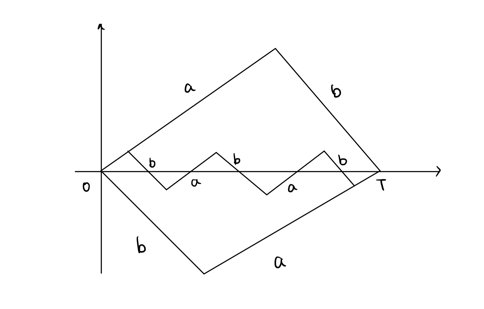
\includegraphics[width=0.8\textwidth]{pics/8-1.png}
        \end{figure}
        So we get the infimum is $0$, and the minimum is $0$ if we allow for any Lipschitz function $x$. In fact, all trajectory with slopes between $[a,b]$ are limiting minimizers. This means we are actually dealing with an \textbf{effective Lagrangian} $L_{eff}$ with the hump between $a$ and $b$ flattened out. The effective Lagrangian $L_{eff}$ is the convex envelope of $L$.

        If we had another Lagrangian like the following, could we again look at the convex envelope? 
        \begin{figure}[H]
            \centering
            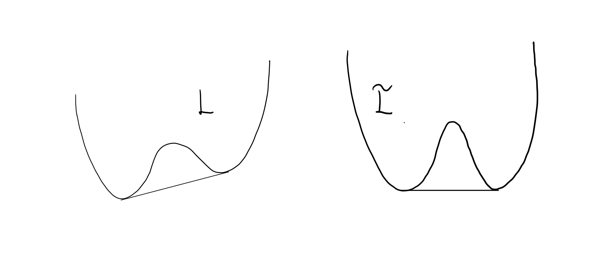
\includegraphics[width=0.8\textwidth]{pics/8-2.png}
        \end{figure}
        Suppose we add a linear constant to get $\widetilde{L}(q) = L+c\cdot q$ and we can get $\widetilde{L}$ as this. So the effective Lagrangian must be convex as a function of $q$. For PDEs, convexity is no longer required. Instead, we require \textbf{rank one convexity}, which is given by convexity in one variable at a time.
    \end{itemize}
\end{remark}

\begin{example}
    Here is an example that comes from classical mechanics. Suppose we have a particle with trajectory $x(t)$ moving in a conservative force field $F = \nabla \phi$, where $\phi$ is the potential. Then we have the Lagrangian 
    \[
        L(x, q)=\underbrace{\frac{1}{2} m q^{2}}_{\text {kinetic energy }}-\underbrace{\phi(x)}_{\text {potential energy }},
    \] 
    where we have $\phi(x) = \frac{d}{dt}(m\dot x)$ ( This comes from the minimizer condition), which we can write as $m\cdot \ddot x = F(x)$, which is Newton's law.
\end{example}

\subsection{Connecting the Hamilton-Jacobi equations to the Euler Lagrange equations}
Returning to Hamilton-Jacobi equations, we have $x,p$ with the function $H$, and we want to relate this to the $x, q=\dot x$ and $L$ in the Euler-Lagrange equation. We can think of the Euler-Lagrange equation as a system for $x$ and $q$ via 
\[
\begin{cases}
    \dot x = q\\
    \frac d {dt} L_q(x,q) = L_x.
\end{cases}
\]
We want to let $p= L_q(x,q)$. For this to make sense, we need $q\to L_q(x,q)$ to be a diffeomorphism from $\RR^n\to \RR^n$ for fixed $x$.

\begin{proposition}
If $L(\cdot) := L(x,\cdot):\RR^n \to \RR$ is strictly convex and coercive ( $\lim_{q\to \infty} \frac{L(x,q)}{|q|} = \infty$), then $p\to L_q(x,p)$ is a diffeomorphism.
\end{proposition}

\begin{proof}
    Injectivity: $L$ is strictly convex, so the graph of $L$ is above its tangent lines at points of nonintersection: 
    \[
        L(y)>L(x)+(y-x) D L(x), \quad y \neq x.
    \]
    We  can use this to write 
    \[
        (y-x)(D L(y)-D L(x))>0, \quad y \neq x.
    \]
    This gives injectivity.
    Surjectivity: We want to minimize $L(x,q)-p\cdot q$. If a minimum exists, then the gradient must equal $0$: 
    \[
        L_q(x,q) = p,
    \]
    which is our surjectivity. Why mut the minimum exist? This is because $\lim_{q\to \infty}L(x,q) - p\cdot q = \infty$ by coercivity. 
    To check that this is a local diffeomorphism, the differential of $q \to L_q(x,q)$ is $L_{qq} \ge 0$. In fact, by strict convexity, this is $>0$. 
    \qed 
\end{proof}

So we have $p=L_q(x,q)$, we will define $H(x,p) = max_{q} p\cdot q - L(x,q)$. Note that this is the same quantity we dealt with in the above proof. The functions $p\cdot q -L(x,q)$ are linear in $p$, so this maximum is convex.

\begin{proposition}
    H is convex and coercive.
\end{proposition}
\begin{proof}
    This comes from the strict convexity and coercivity of $L$. \qed 
\end{proof}
\begin{proposition}
    \[
        q = H_p(x,p).
    \]
\end{proposition}

\begin{proof}
    Since $H$ is defined by maximum, we have $H(x,p)+ L(x,q) -pq \le 0$ and this holds with equality if $p=L_q(x,q)$. Now we can fix q and vary $p$! Then $p$ is a maximum point for this expression when the derivative $H_p(p) -q = 0$. \qed 
\end{proof}

Now let's change our variables: The Euler-Lagrange equations say 
\[
    L_x(x,q) - \frac{d}{dt}\underbrace{L_q(x,q)}_{p} = 0
\]
So we get 
\[
    \left\{\begin{array}{l}
        \dot{p}=L_{x}(x, q) \stackrel{?}{=}-H_{x}(x, p) \\
        \dot{x}=q=H_{p}(x, p)
        \end{array}\right.
\]
We also have 
\[
    H(x,p)+ L(x,q) -pq \le 0.
\]
If we think of $p=p(x,q)$, we can take $\frac{d}{dx}$ to get 
\begin{align*}
    &H_x(x,p) + H_p(x,p) \frac{\partial p}{\partial x} +L_x(x,q) - q\cdot \frac{\partial p}{\partial x}\\
    =& H_x(x,p) + +L_x(x,q) +\underbrace{(H_p(x,p) - q)}_{=0}\cdot \frac{\partial p}{\partial x}=0
\end{align*}
And this tells us that
\[
    L_x(x,q) = -H_x(x,p).
\]
